\documentclass[a4paper]{report}
\usepackage[T1]{fontenc}
\usepackage[utf8]{inputenc}
\usepackage{lmodern}
\usepackage{graphicx}
\usepackage[left=3cm,right=3cm,top=3cm,bottom=3cm]{geometry}
\usepackage{eurosym}
\usepackage{fancyhdr}%encabezado y pie de página
\usepackage[colorlinks=true, linkcolor=black, urlcolor=blue]{hyperref}
\setcounter{secnumdepth}{5}
\usepackage[spanish]{babel}
\setcounter{tocdepth}{5}
\usepackage{colortbl}%para colorear tablas
\usepackage{tabularx}
\usepackage{pdfpages}%para incluir documentos pdf
\usepackage{placeins}%para poner barrera y no pasen de secciones los elemntos flotantes
\usepackage{longtable}
\usepackage{multirow} %para juntar varias filas en una tabla

\author{Andoni Martín Reboredo \\ David Ramirez Ambrosi}
\title{\begin{center}
\textbf{\Huge{Práctica 6, Clustering}} \\ 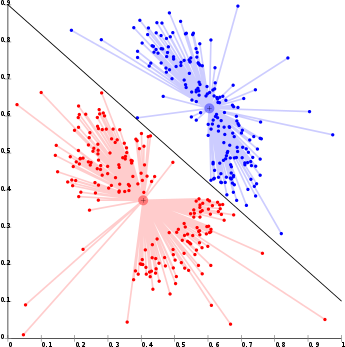
\includegraphics{./Figuras/KMeans-density-data.png}\\  \textbf{Minería de datos}
\end{center}}
\date{\today}



\pagestyle{fancy}
\rhead{
\textbf{Minería de datos} \hfill Práctica 6: Clustering
}

\lhead{}

%colores
\definecolor{azul}{RGB}{0,240,255}
\definecolor{amarillo}{RGB}{255,240,0}
\definecolor{rojo}{RGB}{255,198,198}

%Separación entre párrafos
\setlength{\parskip}{4mm}

\begin{document}
\maketitle

\thispagestyle{empty}%para evitar enumeración de la página de la portada y del índice
\newpage
\tableofcontents%índice
\thispagestyle{empty}
\newpage

\listoffigures%índice de figuras
\thispagestyle{empty}
\newpage

\setcounter{page}{1}%Para reinizar el contador de páginas en la página deseada


\chapter{Introducción}

El presente documento constituye el resultado de la práctica realizada en base a la implementación del algoritmo de clasificación no supervisada \textbf{KPor otra parte, Means clustering}. Este algoritmo trata el agrupamiento de un conjunto de instancias en base a su proximidad con las demás instancias contenidas en el espacio de muestra proporcionado al algoritmo para su ejecución.

Dentro del algoritmo cabe el estudio de diferentes variaciones en los distintos parámetros de que dispone. Nosotros hemos considerado variaciones sobre dos parámetros, el método de cálculo de la distancia entre los distintos elementos que posee el cluster y la inicialización de los distintos clusters, esta inicialización servirá como base de las sucesivas iteraciones que conforman el algoritmo.

	\section{Clasificación no-supervisada}
	La clasificación no supervisada es aquella que se lleva a cabo mediante el estudio de las diversas instancias que conforman el espacio de aplicación del algoritmo sin que estas instancias tengan que estar previamente clasificadas dentro de una clase.
	
	Se trata de una técnica de exploración de los datos en la que se intentan detectar estas clases desconocidas. Dependiendo de el algoritmo de clasificación utilizado, el número de clases debe o no ser especificado. Por ejemplo, en el algoritmo en que se basa este trabajo debe ser especificado, sin embargo en técnicas de \textbf{clusterig jerárquico} no.
	
	\section{Objetivo}
	
	Esta práctica tiene como objetivo principal la comprehensión de los procesos internos que realiza un algoritmo de agrupamiento cualquiera como puede ser el KMeans clustering. El aprendizaje se realizará de forma práctica a través de la creación de un KMeans clustering al que se le añadirán pequeñas variaciones en sus parámetros que deberemos crear.	Estas variaciones requieren que el algoritmo sea entendido plenamente para poder hacer adiciones que tengan un mínimo de sentido.
\chapter{Algoritmo}

	\section{K-means, algoritmo principal}
	
	\begin{verbatim}
	inicializar
	divergencia = infinito 
	
	Mientras(numiteraciones <= iteracionesIndicadas AND divergencia < delta)
	{
	    centroides = centroidesNuevos 
	
	    calcularPertenencias
	    centroidesNuevos = calcularNuevosCentroides
		
	    calcularDivergencia(centroidesNuevos) 
	}
	\end{verbatim}
	
	\section{Subrutina inicialización}
		\subsection{Inicialización aleatoria}
			\begin{verbatim}
			Para cada dimensión
			{
			   mientras extraiga una instancia ya evaluada
			   {
			      extraigo una instancia nueva
			   }
			   añado la instancia extraida a las evaluadas
			   establezco la instancia como centroide de un cluster
			}
			\end{verbatim}
		
		\subsection{Pertenencia aleatoria}
			\begin{verbatim}
			Mientras haya instancias que asignar
			{
			   Calculo un número de cluster aleatorio
			   Extraigo la siguiente instancia
			   Añado la instancia al cluster aleatorio
			}
			Calculo los centroides del cluster
			\end{verbatim}
		
		\subsection{División de espacio}
			\begin{verbatim}
			Obtengo los rangos máximos y mínimos de cada subespacio
			Mientras no haya creado k divisiones
			{
			   Mientras no haya establecido todos los atributos(recorrido los subespacios)
			   {
			      Divido el subespacio en K
			      Asigno el centro del subespacio dividido correspondiente al índice del bucle
			   }
			   Añado el centroide resultante de dividir el espacio
			}
			\end{verbatim}
		
		\subsection{Generación aleatoria de codewords}
		\begin{verbatim}
		Obtengo los máximos y mínimos de cada dimensión
		Para cada cluster
		{
		   Evaluo cada dimensión
		   {
		      Calculo un valor aleatorio para ese centroide en esa dimensión
		   }
		   Añado el centroide generado al cluster
		}
		\end{verbatim}
	\section{Subrutina calcularPertenencias}
	
		\begin{verbatim}
		Crear nuevos clusters 
		
		Para cada instancia
		{
		    Para cada centroide
		    {
		        distancia entre la instancia y cada cluster
		        Guardamos los mínimos 
		    }    
		    Para cada centroide obtenido
		        Guardamos la instancia en el cluster correspondiente al centroide
		}
		\end{verbatim}
	
	\section{Subrutina calcularCentroides}
	
		\begin{verbatim}
		Para cada cluster
		
		   Calcular la instancia media
		   
		return nuevosCentroides
		\end{verbatim}
	
	\section{Subrutina calcularDivergencia}
	
		\begin{verbatim}
		Para cada cluster 
		   
		   Calcular la distancia entre el centroide antiguo y el nuevo
		   
		return divergenciaAcumulada
		\end{verbatim}

\chapter{Diseño}



\chapter{Resultados experimentales}

	\section{Banco de pruebas para la validación de software y resultados}
	
	\section{Resultados}
	
	\section{Clasificación supervisada respecto de otro software de refernecia}
	
	\section{Análisis crítico y discusión de resultados}
	
	\section{Rendimiento del software}

\chapter{Conclusiones}

	\section{Motivación para la realización de clustering \textit{Clustering}}
	
	\section{Conclusiones de los resultados}
	
	\section{Conclusiones generales}
	
	\section{Propuestas de mejora}

%Bibliografía

\newpage
\bibliographystyle{plain}

\bibliography{mdp6}

\chapter{Valoración subjetiva}
	
	\section*{Alcance de objetivos}
	
	\section*{Utilidad de la tarea}
	
	\section*{Dificultad}
	
	\section*{Tiempo de trabajo}
	
	\section*{Sugerencias de mejora}
	
	\section*{Críticas}

\end{document}